\documentclass[11pt]{article}
\usepackage[utf8]{inputenc}
\usepackage[T1]{fontenc}
\usepackage{amsmath}
\usepackage{amssymb} % Needed for \eth
\usepackage{graphicx}
\usepackage{geometry}
\usepackage{tikz}
\usepackage{pgfplots} % For plots
\usepackage{ulem}     % For underline, using normalem to avoid messing with \emph
\usepackage{tcolorbox} % For boxing equations if needed
\usepackage{braket}    % For QM state notation if needed

\geometry{a4paper, margin=1in}
\usetikzlibrary{positioning, arrows.meta, shapes.geometric, patterns, calc} % Added calc library
\pgfplotsset{compat=1.18} % Use a recent PGFPlots version

% Custom commands (optional)
\newcommand{\avg}[1]{\overline{#1}}
\newcommand{\prob}[1]{P(#1)}
\newcommand{\ProbDens}[1]{\mathcal{P}(#1)} % Using script P for density
\newcommand{\vect}[1]{\vec{#1}}
\newcommand{\dd}[1]{\mathrm{d}#1} % Differential d
\newcommand{\pderiv}[2]{\frac{\partial #1}{\partial #2}}
\newcommand{\deriv}[2]{\frac{\mathrm{d} #1}{\mathrm{d} #2}}
\newcommand{\muState}{\mu\text{-state}} % Microstate
\newcommand{\OmegaE}{\Omega(E)}
\newcommand{\omegaE}{\omega(E)}
\newcommand{\PhiE}{\Phi(E)}
\newcommand{\deltaE}{\delta E}
\newcommand{\ethbar}{\text{\it{đ}}} % \eth symbol for inexact differential
\newcommand{\kb}{k_B} % Boltzmann constant (set to 1 for calculations, unless specified)
\newcommand{\gasR}{R} % Ideal gas constant
\newcommand{\partfn}{Z} % Partition function symbol
\newcommand{\grandpartfn}{\mathcal{Z}} % Grand partition function symbol (using \mathcal{Z})
\newcommand{\lambdaT}{\lambda_{th}} % Thermal wavelength
\newcommand{\eps}{\epsilon}
\newcommand{\nbar}{\overline{n}} % Mean occupation number
\newcommand{\ef}{\epsilon_F} % Fermi energy
\newcommand{\kf}{k_F} % Fermi wavevector
\newcommand{\tf}{T_F} % Fermi temperature

\title{Physics 415 - Lecture 32: Fermi Gas}
\date{April 11, 2025}
\author{} % Author not specified

\begin{document}

\maketitle
\thispagestyle{empty}

\section*{Summary}

\begin{itemize}
    \item Fermi-Dirac (FD) statistics: Mean occupation number $\nbar_r = \frac{1}{e^{\beta(\eps_r-\mu)} + 1}$. Grand Potential $\Phi = -T \sum_r \ln(1 + e^{-\beta(\eps_r-\mu)})$.
    \item Density of States (DOS) for free particles (spin $J$, degeneracy $g=2J+1$) in volume $V$:
    \[ \sum_r \to g \int d\eps \, \rho(\eps) \]
    where $\rho(\eps) = \frac{V}{4\pi^2} \left( \frac{2m}{\hbar^2} \right)^{3/2} \sqrt{\eps}$. $\rho(\eps)d\eps =$ \# of spatial states in energy range $(\eps, \eps+d\eps)$.
\end{itemize}
So far, we developed the general theory of ideal QM gases. Now focus on the specific case of FD statistics.

\section*{Fermi Gas (FG)}

A system of non-interacting fermions.
Examples: conduction electrons ($e^-$) in a metal, white dwarf stars, neutron stars, liquid $^3$He, ...

The mean occupation number $\nbar(\eps)$ plays a central role:
\[ \nbar(\eps) = \frac{1}{e^{\beta(\eps-\mu)} + 1} \quad (\text{Fermi function}) \]

\subsection*{Fermi Gas at T=0}

At $T=0$ ($\beta \to \infty$), the FG will be in its QM ground state. Due to the Pauli exclusion principle, fermions successively fill up the single-particle states starting from the lowest energy.
The Fermi function becomes a step function:
\[ \lim_{T \to 0} \nbar(\eps) = \begin{cases} 1 & \text{if } \eps < \mu(T=0) \\ 0 & \text{if } \eps > \mu(T=0) \end{cases} \]
The chemical potential at $T=0$ is called the \textbf{Fermi energy}, denoted by $\ef \equiv \mu(T=0)$. It is the energy of the highest occupied state at $T=0$.

\begin{center}
\begin{tikzpicture}
\begin{axis}[
    xlabel={Energy $\epsilon$}, ylabel={Mean Occupation $\overline{n}(\epsilon)$},
    xmin=0, ymin=0, ymax=1.2,
    axis lines=left,
    xtick = {2}, xticklabels = {$\mu=\epsilon_F$},
    ytick = {1},
    title = {Fermi function at T=0}
]
\addplot [domain=0:2, thick, blue, const plot] {1};
\addplot [domain=2:5, thick, blue, const plot] {0};
\draw [thick, blue] (axis cs:2, 1) -- (axis cs:2, 0); % Vertical line at Ef
\end{axis}
\end{tikzpicture}
\end{center}

The filled states with $\eps < \ef$ form the \textbf{"Fermi sea"}.
In $\vec{k}$-space, the Fermi sea corresponds to filling all $\vec{k}$ states up to a limiting wave-vector $k_F$ (Fermi wave-vector). The surface $|\vec{k}| = k_F$ is the \textbf{Fermi surface}.
Relation: $\ef = \frac{\hbar^2 k_F^2}{2m}$. The Fermi momentum is $p_F = \hbar k_F$.

\begin{center}
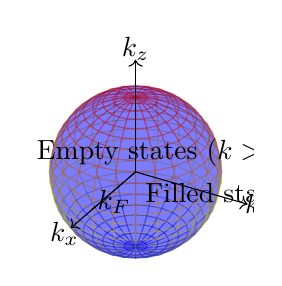
\begin{tikzpicture}
\begin{axis}[
    xlabel=$k_x$, ylabel=$k_y$, zlabel=$k_z$,
    view={120}{30},
    axis equal image,
    hide axis,
]
% Draw sphere
\addplot3 [surf, opacity=0.3, blue, z buffer=sort, domain=0:360, y domain=0:180] ({2*cos(x)*sin(y)}, {2*sin(x)*sin(y)}, {2*cos(y)});
% Draw axes
\draw [->] (0,0,0) -- (3,0,0) node [pos=1.1] {$k_x$};
\draw [->] (0,0,0) -- (0,3,0) node [pos=1.1] {$k_y$};
\draw [->] (0,0,0) -- (0,0,3) node [pos=1.1] {$k_z$};
% Label radius
\draw [dashed] (0,0,0) -- (2,0,0);
\node at (1,0,-0.3) {$k_F$};
% Label filled/empty
\node at (0,0,0) [below right] {Filled states ($k<k_F$)};
\node at (2.5, 2.5, 2.5) {Empty states ($k>k_F$)};
\end{axis}
\end{tikzpicture}
\end{center}

The Fermi wave-vector $k_F$ (and hence $\ef$) is determined by the total particle number $N$:
\[ N = \sum_r \nbar_r \xrightarrow{T=0} \sum_{r \text{ with } \eps_r < \ef} (g \times 1) \]
Using the integral form:
\[ N = g V \int_{k < k_F} \frac{d^3k}{(2\pi)^3} \]
The integral is the volume of a sphere of radius $k_F$ in k-space, which is $\frac{4}{3}\pi k_F^3$.
\[ N = g V \frac{1}{(2\pi)^3} \left( \frac{4}{3}\pi k_F^3 \right) = \frac{g V k_F^3}{6\pi^2} \]
The particle density is $n = N/V = \frac{g k_F^3}{6\pi^2}$.
\[ k_F = \left( \frac{6\pi^2 n}{g} \right)^{1/3} \]
The Fermi energy is:
\[ \ef = \frac{\hbar^2 k_F^2}{2m} = \frac{\hbar^2}{2m} \left( \frac{6\pi^2 n}{g} \right)^{2/3} \]
(For electrons, spin $J=1/2$, so $g=2J+1=2$. $k_F = (3\pi^2 n)^{1/3}$).

Alternatively, use the DOS $\rho(\eps)$:
\[ N = g \int_0^{\ef} \rho(\eps) d\eps \quad (\text{since } \nbar=1 \text{ for } \eps < \ef, 0 \text{ otherwise}) \]
\[ N = g \left( \frac{V}{4\pi^2} \left(\frac{2m}{\hbar^2}\right)^{3/2} \right) \int_0^{\ef} \sqrt{\eps} d\eps = \frac{gV}{4\pi^2} \left(\frac{2m}{\hbar^2}\right)^{3/2} \left[ \frac{2}{3}\eps^{3/2} \right]_0^{\ef} \]
\[ N = \frac{gV}{6\pi^2} \left(\frac{2m}{\hbar^2}\right)^{3/2} \ef^{3/2} \]
Solving for $\ef$: $\ef^{3/2} = \frac{6\pi^2 N}{gV} \left(\frac{\hbar^2}{2m}\right)^{3/2}$.
\[ \ef = \left( \frac{6\pi^2 n}{g} \right)^{2/3} \left( \frac{\hbar^2}{2m} \right) \checkmark \]

It is useful to express the DOS at the Fermi energy, $\rho(\ef)$, in terms of $N$ and $\ef$.
From $N = \frac{2}{3} g (AV\ef^{1/2}) \ef$ where $AV\ef^{1/2} = \rho(\ef)$:
$N = \frac{2}{3} g \rho(\ef) \ef$.
\[ \rho(\ef) = \frac{3 N}{2 g \ef} \]

\textbf{Total Energy at T=0 ($E_0$):}
\[ E_0 = \sum_r \nbar_r \eps_r = g \int_0^{\ef} \rho(\eps) \eps d\eps \]
\[ E_0 = g \left( \frac{V}{4\pi^2} \left(\frac{2m}{\hbar^2}\right)^{3/2} \right) \int_0^{\ef} \eps^{3/2} d\eps \]
\[ E_0 = g A V \left[ \frac{2}{5}\eps^{5/2} \right]_0^{\ef} = \frac{2}{5} g A V \ef^{5/2} \]
Substitute $g A V = \frac{3N}{(2/3)\ef^{3/2}}$? No, substitute $gAV = \frac{3N}{(2/3)\ef^{3/2}} \times \frac{2}{3} = \frac{3N}{\ef^{3/2}}$.
$E_0 = \frac{2}{5} \left( \frac{3N}{\ef^{3/2}} \right) \ef^{5/2} = \frac{3}{5} N \ef$.
The total energy $E_0 = \frac{3}{5} N \ef$ is non-zero even at $T=0$. This is purely a QM effect due to the Pauli principle. (Classical ideal gas has $E=0$ at $T=0$).

\textbf{Pressure at T=0 ($p_0$):}
Using the general relation $pV = \frac{2}{3}E$ for non-relativistic free particles:
\[ p_0 = \frac{2}{3} \frac{E_0}{V} = \frac{2}{3V} \left( \frac{3}{5} N \ef \right) = \frac{2}{5} \frac{N}{V} \ef = \frac{2}{5} n \ef \]
The pressure of a Fermi gas is non-zero even at $T=0$. This is the "degeneracy pressure", arising from the kinetic energy forced upon the fermions by the exclusion principle. (Classical ideal gas $p=nT \to 0$ as $T \to 0$).

\subsection*{Fermi Gas at T>0}

The important temperature scale is the Fermi energy $\ef$ (or Fermi temperature $\tf = \ef / \kb$).
\begin{itemize}
    \item Low-T "degenerate" regime: $T \ll \tf$. Quantum effects dominate. Condition $n\lambdaT^3 \gg 1$.
    \item High-T "non-degenerate" regime: $T \gg \tf$. Classical limit applies. Condition $n\lambdaT^3 \ll 1$.
\end{itemize}
For electrons in metals, $\tf \sim 10^4 - 10^5$ K. So at room temperature ($T \approx 300$ K), they are highly degenerate and QM effects dominate.

Consider the Fermi function $\nbar(\eps)$ for $0 < T \ll \tf$.
The step function at $T=0$ broadens into a smooth curve over an energy range of order $T$ (or $\kb T$) around $\eps = \mu$. For $T \ll \tf$, the chemical potential $\mu$ is only slightly different from $\ef$.

\begin{center}
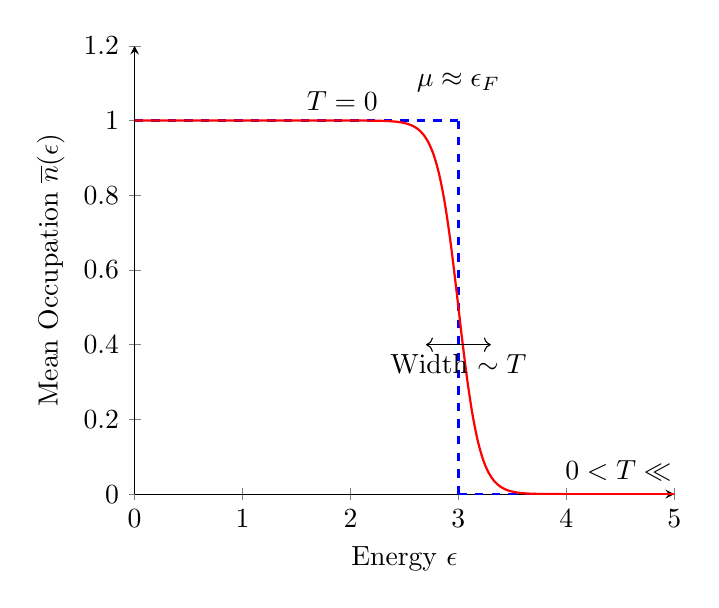
\begin{tikzpicture}
\begin{axis}[
    xlabel={Energy $\epsilon$}, ylabel={Mean Occupation $\overline{n}(\epsilon)$},
    xmin=0, ymin=0, ymax=1.2,
    axis lines=left,
    legend pos=outer north east
]
% T=0
\addplot [domain=0:3, thick, blue, dashed] {1} node [pos=0.5, above right, black] {$T=0$};
\addplot [domain=3:5, thick, blue, dashed] {0};
\draw [thick, blue, dashed] (axis cs:3, 1) -- (axis cs:3, 0);
\node at (axis cs:3, -0.05) {$\ef$};

% T > 0 (e.g., T ~ 0.1 Ef) => beta ~ 10/Ef. mu approx Ef=3.
\addplot [domain=0:5, samples=100, smooth, thick, red] {1/(exp(10*(x-3))+1)} node [pos=0.8, above right, black] {$0 < T \ll T_F$};

% Transition region width
\draw [<->] (axis cs:2.7, 0.4) -- (axis cs:3.3, 0.4) node [midway, below] {Width $\sim T$};
\node at (axis cs:3, 1.05) [anchor=south, black] {$\mu \approx \ef$};
\end{axis}
\end{tikzpicture}
\end{center}

Qualitatively: When $T \ll \tf$, only particles within an energy range of order $T$ near the Fermi surface ($\eps \approx \ef$) can be thermally excited into available empty states just above $\ef$. States deep in the Fermi sea ($\eps \ll \ef$) are "blocked" by occupied states above them (Pauli exclusion).

The "effective" number of particles that participate in thermal activity is approximately:
\[ N_{eff} \approx (\text{Density of states near } \ef) \times (\text{Energy range}) \]
\[ N_{eff} \sim \rho(\ef) \times T \]
Using $\rho(\ef) \sim N/\ef$:
\[ N_{eff} \sim \frac{N}{\ef} T = N \left( \frac{T}{\tf} \right) \]
Since $T \ll \tf$, $N_{eff} \ll N$. Only a small fraction of fermions contribute to thermal properties like heat capacity at low T.

\subsection*{Low Temperature Thermodynamics (Estimates)}

Estimate the energy $E(T)$ at low T:
$E(T) \approx E_0 + (\text{Energy added to excited particles})$.
Each of the $N_{eff}$ particles gains roughly energy $T$.
\[ E(T) \approx E_0 + N_{eff} \times T \sim E_0 + N \left( \frac{T}{\tf} \right) T = E_0 + \frac{N T^2}{\tf} \]
(Here $T, \tf$ are in energy units).
Heat capacity $C_V$:
\[ C_V = \left( \pderiv{E}{T} \right)_V \sim \pderiv{}{T} \left( E_0 + \frac{N T^2}{\tf} \right) = \frac{2N T}{\tf} \sim N \left( \frac{T}{\tf} \right) \]
So $C_V \propto T$ at low temperatures.

\begin{center}
\begin{tikzpicture}
\begin{axis}[
    xlabel={$T$}, ylabel={$C_V$},
    xmin=0, ymin=0,
    xtick=\empty, ytick=\empty,
    axis lines=left, width=7cm, height=4cm,
    legend pos=north west
]
\addplot [domain=0:3, samples=100, smooth, thick, blue] {1.5*x} node[pos=0.7, anchor=west] {$C_V \propto T$}; % Low T linear behavior
\addplot [domain=2:5, dashed, thick, red] {4.5} node[pos=0.5, anchor=south] {Classical $C_V = \frac{3}{2}N$}; % High T classical limit
\draw [dotted] (axis cs:2,0) node[below]{$T_F$} -- (axis cs:2, 4.5);
\end{axis}
\end{tikzpicture}
\end{center}
This linear dependence $C_V \propto T$ is characteristic of degenerate Fermi gases (e.g., electron contribution in metals) and contrasts sharply with the classical result ($C_V = \frac{3}{2}N k_B$, constant) or lattice vibrations ($C_V \propto T^3$).

To make these estimates more precise requires evaluating integrals of the form
\[ I = \int_0^\infty d\eps \, f(\eps) \nbar(\eps) = \int_0^\infty d\eps \frac{f(\eps)}{e^{\beta(\eps-\mu)}+1} \]
in the degenerate regime $T \ll \tf$. This involves the Sommerfeld expansion (next lecture).

\end{document}